\subsection{Motivation}
	The three main terms of the title of this work are Text annotation, assistance and evaluation. To motivate and explain the relation of these terms, we are going to have a look at their meaning.

	\begin{figure}[h]
		\centering
		\subfloat[Apple Siri]{{
			
\includegraphics[width=2cm]{assets/1/AppleSiri.png}
		}}
		\qquad
		\subfloat[Google Home]{{
			
\includegraphics[width=2cm]{assets/1/GoogleHome.png}
		}}
		\qquad
		\subfloat[Facebook M]{{
			
\includegraphics[width=2cm]{assets/1/FacebookM.png}
		}}
		\qquad
		\subfloat[Amazon Alexa]{{
			
\includegraphics[width=2cm]{assets/1/AmazonAlexa.png}
		}}
		\qquad
		\subfloat[Microsoft Cortana]{{
			
\includegraphics[width=2cm]{assets/1/MSCortana.png}
		}}
		\caption{Smart assistants use \ac{ML} to process spoken requests.}%
		\label{fig:exampleHomeAssistants}%
	\end{figure}

	Using \ac{ML} allows data scientists to extract information from huge amounts of data. \ac{NER}, for example, is such an extraction technique: The goal is to identify names of persons, places, groups (like organizations or companies) and other entities in texts. Applications to such technology are for example smart assistances like Siri on the iPhone or Alexa as a standalone device in living rooms. Five of the most popular examples of such assistances are listed in Figure~\ref{fig:exampleHomeAssistants}. They all have in common to first translate speech to text and then process this text to \textit{understand} what it is about. Smart assistances aren't the only field of application, though: Chatbots and spam filters use \ac{NER} as well, to name just a few end user products. This kind of technology is also useful when it comes to the analysis of large amount of data, exceeding the amount humans could process in a reasonable amount of time. Another real world example: Leaks like the Snowden documents of the Panama Papers need to be processed automatically to get an idea of where to start an investigation, since such large scales of text are simply too big to be assessed by an individual in a reasonable amount of time.

	% für nlp braucht man annotierte Daten
	% little ML intro, explain supervised learning
	Tools and techniques that help creating machines capabale of processing natural language text are summarized as \ac{NLP}. The task of automatically recognizing named entities is called \ac{NER}. This lays an important foundation to make machines \textit{understand} human sentences. One way to teach a machine is by presenting both the data that needs to be processed and the result of a processing to it. The \textit{how} can be inferred. An \ac{ML} algorithm tries to generalize the information from the training (the learning phase) and creates a \textit{model}, which will later be used to predict an outcome towards data it has not seen before. In this case it means showing the algorithm texts with correctly annotated entities. This presentation of showing data and labels at once is called \textit{supervised learning}.\footnote{In contrast to \textit{unsupervised learning}. This describes a group of algorithms which try to learn something (like patterns for classification for example) out of unlabeled data.}

	% demand for training data, example of sentence analysis
	It is hard to create a model that reflects complex concepts like understanding a natural language. Figure~\ref{fig:MlTextAnalysis} shows a few of the fundamental steps needed to access the meaning of a rather simple sentence. A common concept to handle hard problems like this is to divide it into several simpler subtasks. The chain of these subtasks is called \textit{pipeline}. The final outcome of such a pipeline depends much on the quality of each of the single steps. This is why good \ac{ML} models depend on good training data -- everything they \lqq know\rqq has been inferred from the training data. If this data doesn't depict a certain aspect of the desired behavior a resulting model has no chance to make correct predictions. Training data is key to the model's performance. In the case of \ac{ML} for \ac{NER} training data are annotated texts.

	\singleFullSizeFig{1/MLSentenceParsing.png}{Exemplary analysis of a simple sentence.}{MlTextAnalysis}

	% das ist text annotation
	\paragraph{Text Annotation} Annotated texts are one or more words or phrases labelled and often highlighted, depending on the \ac{UI}. These annotations have special meanings, abstractly describing the membership of a group. For example to identify names of companies, names of places, addresses or phone numbers -- to name just a few. In this work we are interested in the annotation of named entities, like in the example given in Figure~\ref{fig:exampleAnnotation}:

	\begin{figure}[h]
		\centering
		\subfloat[Plain text]{{
			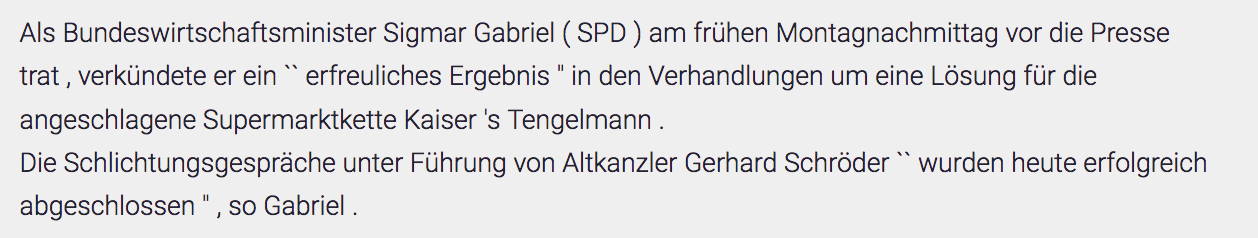
\includegraphics[width=12cm]{assets/1/text-plain.png}
		}}
		\qquad
		\subfloat[Annotated text]{{
			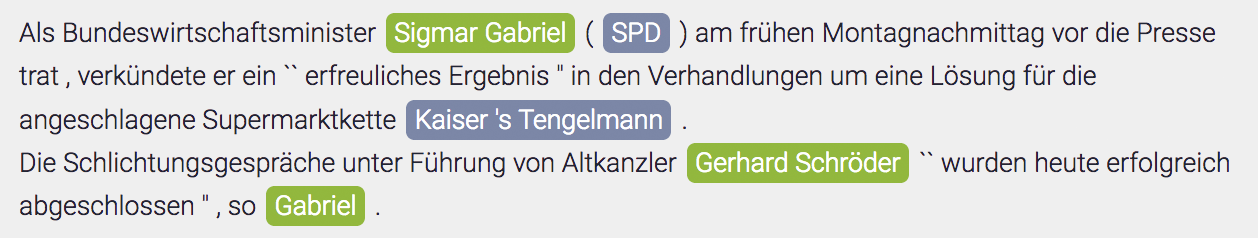
\includegraphics[width=12cm]{assets/1/text-annotated.png}
		}}
		\caption{Example of a German text with and without annotated entities. Green annotations identify person names, blue annotations identify company and organization names.}%
		\label{fig:exampleAnnotation}%
	\end{figure}

	\ac{ML} models working on natural language are most of the time specifically trained for one language, often even for a certain text domain. They work by deriving patterns from their training data. Hence they can not be (usefully) used for an other language. If text domains heavily drift apart from each other in terms of grammar or word use, a model trained on one text domain might not work well on another one, even if both are in the same language. For example, an \ac{NER} model trained on scientific papers used on Twitter tweets will most likely not perform as well as one trained on the appropriate data set -- even though the same algorithm is used.

	To generate different models for different text domains, data scientists need great amounts of different training data sets. Each of them need to be carefully crafted, as correct and complete as possible, allowing the derivation of as much information as possible. This is mostly a manual and thus monotonous and time consuming task -- and therefore it is expensive.
